% Created 2020-11-10 二 23:53
% Intended LaTeX compiler: xelatex
\documentclass[11pt]{article}
\usepackage{graphicx}
\usepackage{grffile}
\usepackage{longtable}
\usepackage{wrapfig}
\usepackage{rotating}
\usepackage[normalem]{ulem}
\usepackage{amsmath}
\usepackage{textcomp}
\usepackage{amssymb}
\usepackage{capt-of}
\usepackage{hyperref}
\usepackage{ctex}
\author{Wang Jian}
\date{\today}
\title{Scaling Distributed Machine Learning With The Parameter Server}
\hypersetup{
 pdfauthor={Wang Jian},
 pdftitle={Scaling Distributed Machine Learning With The Parameter Server},
 pdfkeywords={},
 pdfsubject={},
 pdfcreator={Emacs 27.1 (Org mode 9.4)}, 
 pdflang={English}}
\begin{document}

\maketitle
\tableofcontents

\begin{itemize}
\item OSDI 2014
\end{itemize}
\section{Abstract}
\label{sec:orga1d5c76}
We propose a parameter server framework for distributed machine learning problems. 
\section{1 Introduction}
\label{sec:orgd8995d9}
Sharing imposes three challenges:(带宽、同步、容错)
\begin{itemize}
\item Accessing the parameters requires an enormous amount of network bandwidth.
\item Many machine learning algorithms are sequential. The resulting barriers hurt performance when the cost of synchronization and machine latency is high.
\item At scale, fault tolerance is critical. Learning tasks are often performed in a cloud environment where machines can be unreliable and jobs can be preempted.

\begin{center}
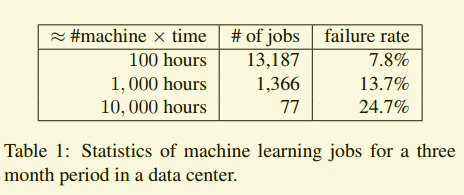
\includegraphics[width=.9\linewidth]{PS.org_imgs/20201108_162123_doWREW.png}
\end{center} 

\uline{对第三点的解释。Here, task failure is mostly due to being preempted or losing machines without necessary fault tolerance mechanisms.}
\end{itemize}
\subsection{1.1 Contributions}
\label{sec:org6a73973}
该文提出第三代的参数服务器。It confers two advantages to developers:
\begin{itemize}
\item enables application-specific code to remain concise
\item \uline{it provides a robust, versatile, and high-performance implementation capable of handling a diverse array of algorithms from sparse logistic regression to topic models and distributed sketching.}

Our parameter server provides five key features: 
\begin{itemize}
\item Efficient communication
\item Flexible consistency models
\item Elastic Scalability
\item Fault Tolerance and Durability
\item Ease of Use
\end{itemize}
\end{itemize}
\subsection{1.2 Engineering Challenges}
\label{sec:orgf81ee8c}
reading and updating parameters shared between different worker nodes is ubiquitous. parameter server 保存部分参数,worker node 需要这些参数的子集。两个挑战:
\begin{itemize}
\item Communication
parameter: key-value pairs, 值通常很小,每次跟新操作开销很大,采用这种方式低效。解决办法:参数通常表示为向量或张量等,
\item Fault tolerance
failover 故障转移,self-repair 能为动态扩展提供支持

\begin{center}
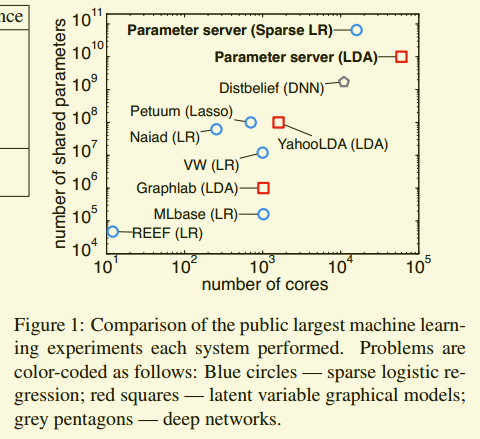
\includegraphics[width=.9\linewidth]{PS.org_imgs/20201109_162042_R64TTN.png}
\end{center} 

\begin{center}
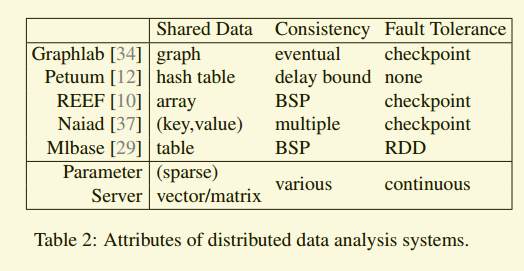
\includegraphics[width=.9\linewidth]{PS.org_imgs/20201109_162533_ZZHIl4.png}
\end{center} 

简而言之,我们的工作比公开的其他工作要好。
\end{itemize}
\subsection{1.3 Related Work}
\label{sec:org9a0ee71}
发展历程:
\begin{itemize}
\item The first generation of such parameter servers: memcached distributed(key, value) store
\item The second generation: Distbelief
\item The third generation: Ours
\end{itemize}

其他:
\begin{itemize}
\item GraphLab 缺乏弹性的可扩展性
\item Piccolo 使用参数服务器的策略进行多台机器的状态共享和聚合,他因此实现了我们系统的大部分功能,但缺少优化策略(message compression, replication, and variable consistency models expressed via dependency graphs)
\end{itemize}
\section{2 Machine Learning}
\label{sec:org527e603}
\subsection{2.1 Goals}
\label{sec:org8980a79}
目标函数(objective function), 如何快速训练大量的数据是我们的关注的重点。
\subsection{2.2 Risk Minimization}
\label{sec:org456bd8d}
rish -- prediction error, overfit, 正则化, loss, 一些机器学习的概念等等。损失函数和正则化对本文不重要。

\uline{我们简单描述为distributed subgradient descent: 次梯度方面只是简单地推广到损失函数和不需要连续可微的正则化器,如在w = 0的|w|}

\begin{center}
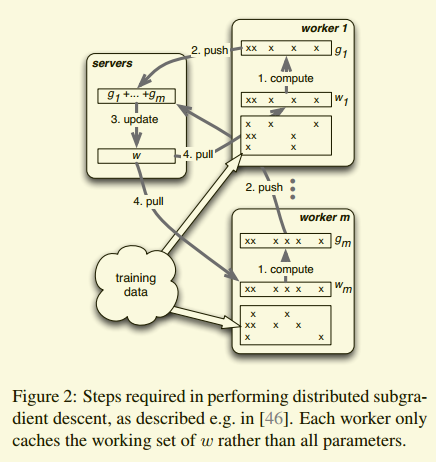
\includegraphics[width=.9\linewidth]{PS.org_imgs/20201109_205205_0B2DJo.png}
\end{center}

每个worker只训练自己的数据,得到subgradient,然后聚集跟新w。

\begin{center}
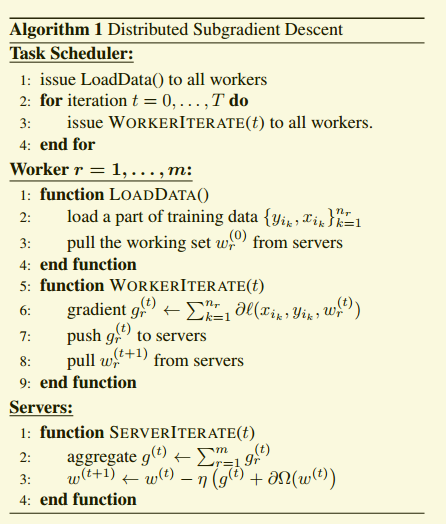
\includegraphics[width=.9\linewidth]{PS.org_imgs/20201109_205231_utqe0Y.png}
\end{center}

时间开销最大的是计算subgradient,但是计算被分配到多台机器。

\begin{center}
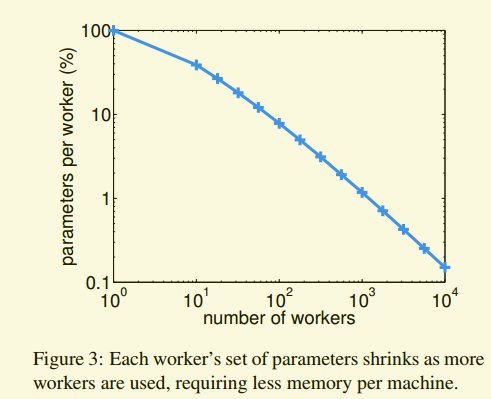
\includegraphics[width=.9\linewidth]{PS.org_imgs/20201110_140316_aTJmHM.png}
\end{center}

worker越多,每个worker上的参数就越少。 \uline{参数不应该是固定数量的吗?网络是全连接的?}
\subsection{2.3 Generative Models}
\label{sec:orgecff44e}
对于无监督学习,算法1需要进行改进,每次跟新不是梯度,而是与文档主题的契合度(topic modeling),同时需要补充信息(单词的含义)。
\section{3 Architecture}
\label{sec:orgadf642a}
\begin{center}
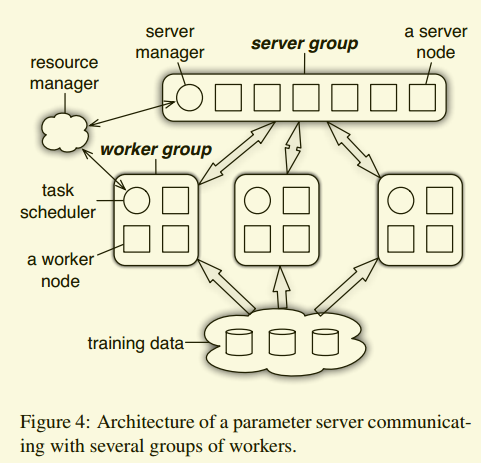
\includegraphics[width=.9\linewidth]{PS.org_imgs/20201110_182452_3VgbEb.png}
\end{center}

每个参数服务器既支持单独的参数空间,又支持共享参数空间。
\subsection{3.1 (Key, Value) vectors}
\label{sec:orgfd9b2f1}
the pair is a feature ID and its weight.
\subsection{3.2 Range Push and Pull}
\label{sec:org1feb1c5}
w.push(R, dest), w.pull(R, dest) 为了编程和效率,支持range-based push and pull
\subsection{3.3 User-Defined Functions on the Server}
\label{sec:orgb613783}
服务器可以执行用户定义的函数
\subsection{3.4 Asynchronous Tasks and Dependency}
\label{sec:orgbe811c7}
\begin{itemize}
\item 任务是同步的:
\begin{itemize}
\item The caller marks a task as finished only once it receives the callee’s reply.
\item The callee marks a task as finished only if the call of the task is returned and all subtasks issued by this call are finished
\end{itemize}
\item 任务以来能提高算法逻辑性和模型的一致性
\end{itemize}
\begin{center}
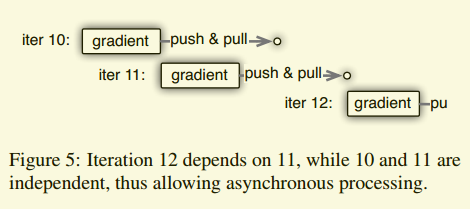
\includegraphics[width=.9\linewidth]{PS.org_imgs/20201110_184541_yCmmwR.png}
\end{center} 

\subsection{3.5 Flexible Consistency}
\label{sec:org1222424}
任务的独立性能提高并行程度,提高系统效率,但是导致不一致性,因此需要trade-off。

关于任务之间的以来可以建立三种模型:Sequential, Eventual, Bounded Delay。值得注意的是,这些图应该是动态的,因为时间是可变的。

\begin{center}
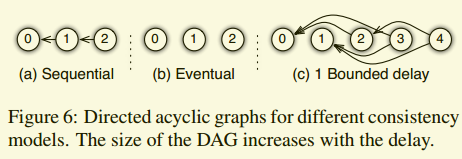
\includegraphics[width=.9\linewidth]{PS.org_imgs/20201110_184713_Wz0I8x.png}
\end{center}
\subsection{3.6 User-defined Filters}
\label{sec:orgd190094}
使用用户定义的过滤器选择需要同步的key-value pairs。KKT: a worker only pushes gradients that are likely to affect the weights on the servers
\section{4 Implementation}
\label{sec:org6e0b2d8}
\subsection{4.1 Vector Clock}
\label{sec:orgefe0b89}
\begin{itemize}
\item 用来记录每个节点(key, value) pair的时间。
\item 许多参数时间戳相同
\end{itemize}
\begin{center}
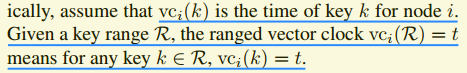
\includegraphics[width=.9\linewidth]{PS.org_imgs/20201110_185915_tUCyTP.png}
\end{center}

\begin{center}
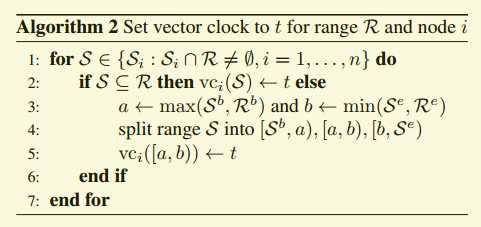
\includegraphics[width=.9\linewidth]{PS.org_imgs/20201110_214651_eJdEsX.png}
\end{center}
\subsection{4.2 Messages}
\label{sec:org8b55c7a}
\begin{center}
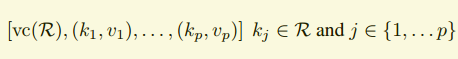
\includegraphics[width=.9\linewidth]{PS.org_imgs/20201110_190122_KcTtuT.png}
\end{center}
参数服务器的基本通信格式,我们使用fast Snappy compression library压缩信息。
\subsection{4.3 Consistent Hashing}
\label{sec:orgc5a7622}
\begin{center}
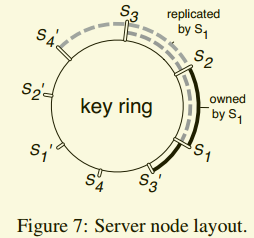
\includegraphics[width=.9\linewidth]{PS.org_imgs/20201110_190423_IeaQJ7.png}
\end{center}
每个服务器节点负责它的开始到下一个节点,该节点是该key range的master。
\subsection{4.4 Replication and Consistency}
\label{sec:org907026c}
\begin{center}
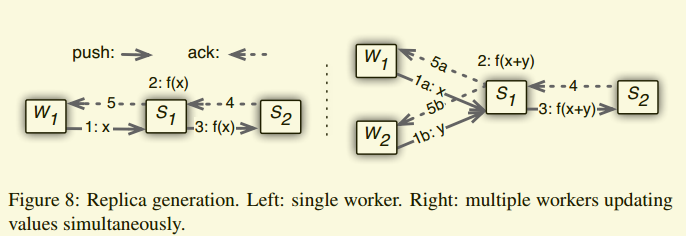
\includegraphics[width=.9\linewidth]{PS.org_imgs/20201110_191114_nNFZVT.png}
\end{center}
过多的复制会影响带宽。
\subsection{4.5 Server Management}
\label{sec:org3533988}
为了提高系统容错和动态扩展能力,我们必须支持添加和删除节点。
\subsection{4.6 Worker Management}
\label{sec:org306c8f4}
添加和删除worker node
\section{5 Evaluation}
\label{sec:org87b3749}
Sparse Logistic Regression and Latent Dirichlet Allocation
\subsection{5.1 Sparse Logistic Regression}
\label{sec:org1521f85}
\begin{itemize}
\item Problem and Data: ad click prediction dataset, 1000 machines
\item Algorithm:
\begin{center}
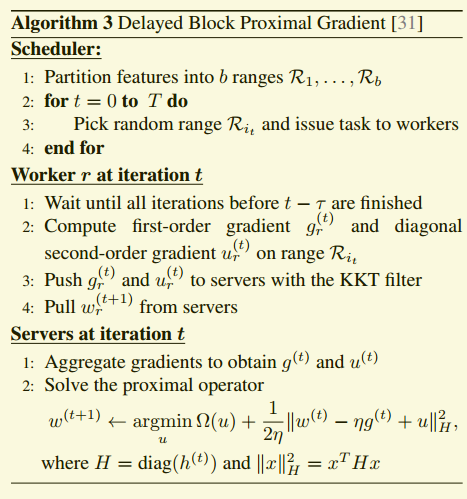
\includegraphics[width=.9\linewidth]{PS.org_imgs/20201110_214356_4k00Hx.png}
\end{center} 
它与之前的有四点不同:
\begin{itemize}
\item 每次迭代只有一部分参数被更新
\item workers 计算梯度和这一部分参数的二阶导数
\item 服务器根据聚集的局部梯度求解近似算子来更新模型
\item bounded-delay model, Karush-Kuhn-Tucker (KKT) filter
\end{itemize}
\item Results:
compare ours with two others, 一些比较结果
\end{itemize}
\subsection{5.2 Latent Dirichlet Allocation}
\label{sec:org5564120}
用户兴趣,LDA
\subsection{5.3 Sketches}
\label{sec:org7208d66}
\ldots{}
\section{6 Summary and Discussion}
\label{sec:org4eeb96d}
\begin{itemize}
\item 提出PS架构
\item 易用:全局参数共享。高效:所有通信都是同步的。灵活的一致性:在效率和算法的收敛速度折中。
\item 弹性扩展和容错
\end{itemize}
\end{document}
